\chapter{Design And Implementation}


\begin{figure}[h]
  \section{DATA FLOW DIAGRAM}
  \centering
  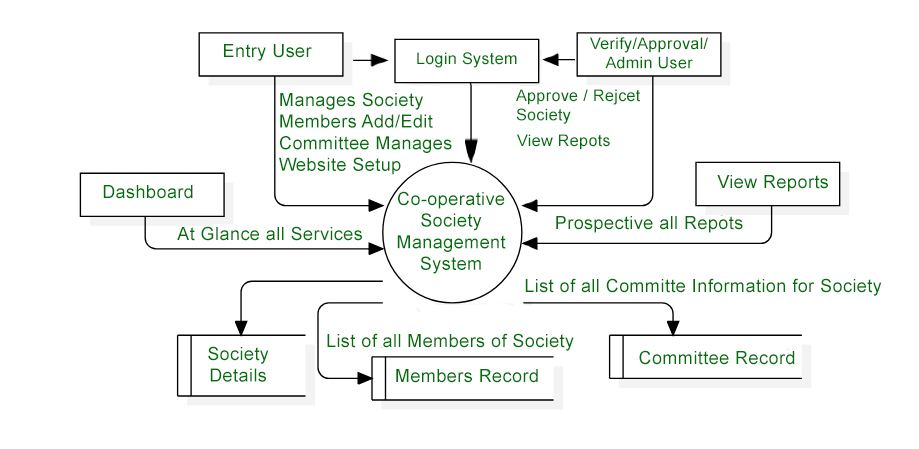
\includegraphics[width=0.6\textwidth]{Chap3/1.jpg}
  \caption{Data Flow Diagram}
  % \label{fig:example}
\end{figure}


\begin{figure}[h]
  \section{USE CASE DIAGRAM}
  \centering
  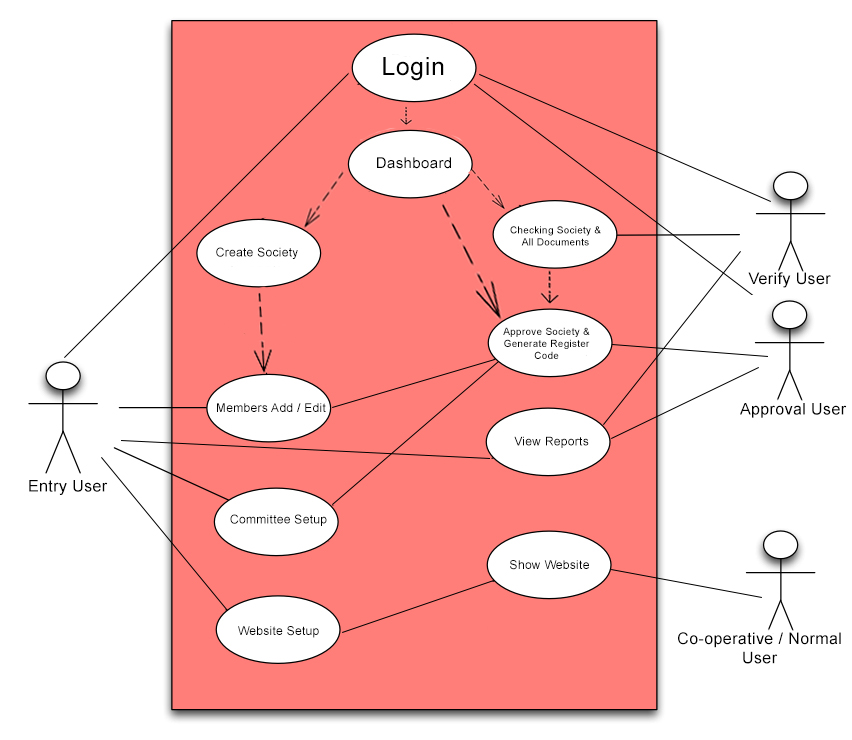
\includegraphics[width=0.6\textwidth]{Chap3/2.jpg}
  \caption{Use Case Diagram}
  \label{fig:example}
\end{figure}

\begin{figure}[h]
\section{PROCESS DIAGRAM}
  \centering
  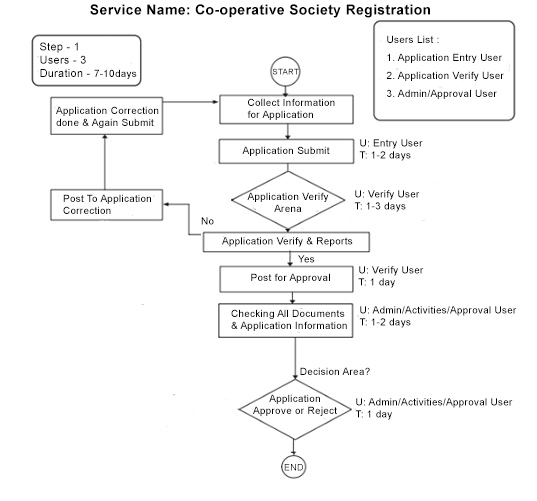
\includegraphics[width=0.6\textwidth]{Chap3/3.png}
  \caption{Process Diagram}
  \label{fig:example}
\end{figure}

\begin{figure}[h]
\section{ENTRY USER}
  \centering
  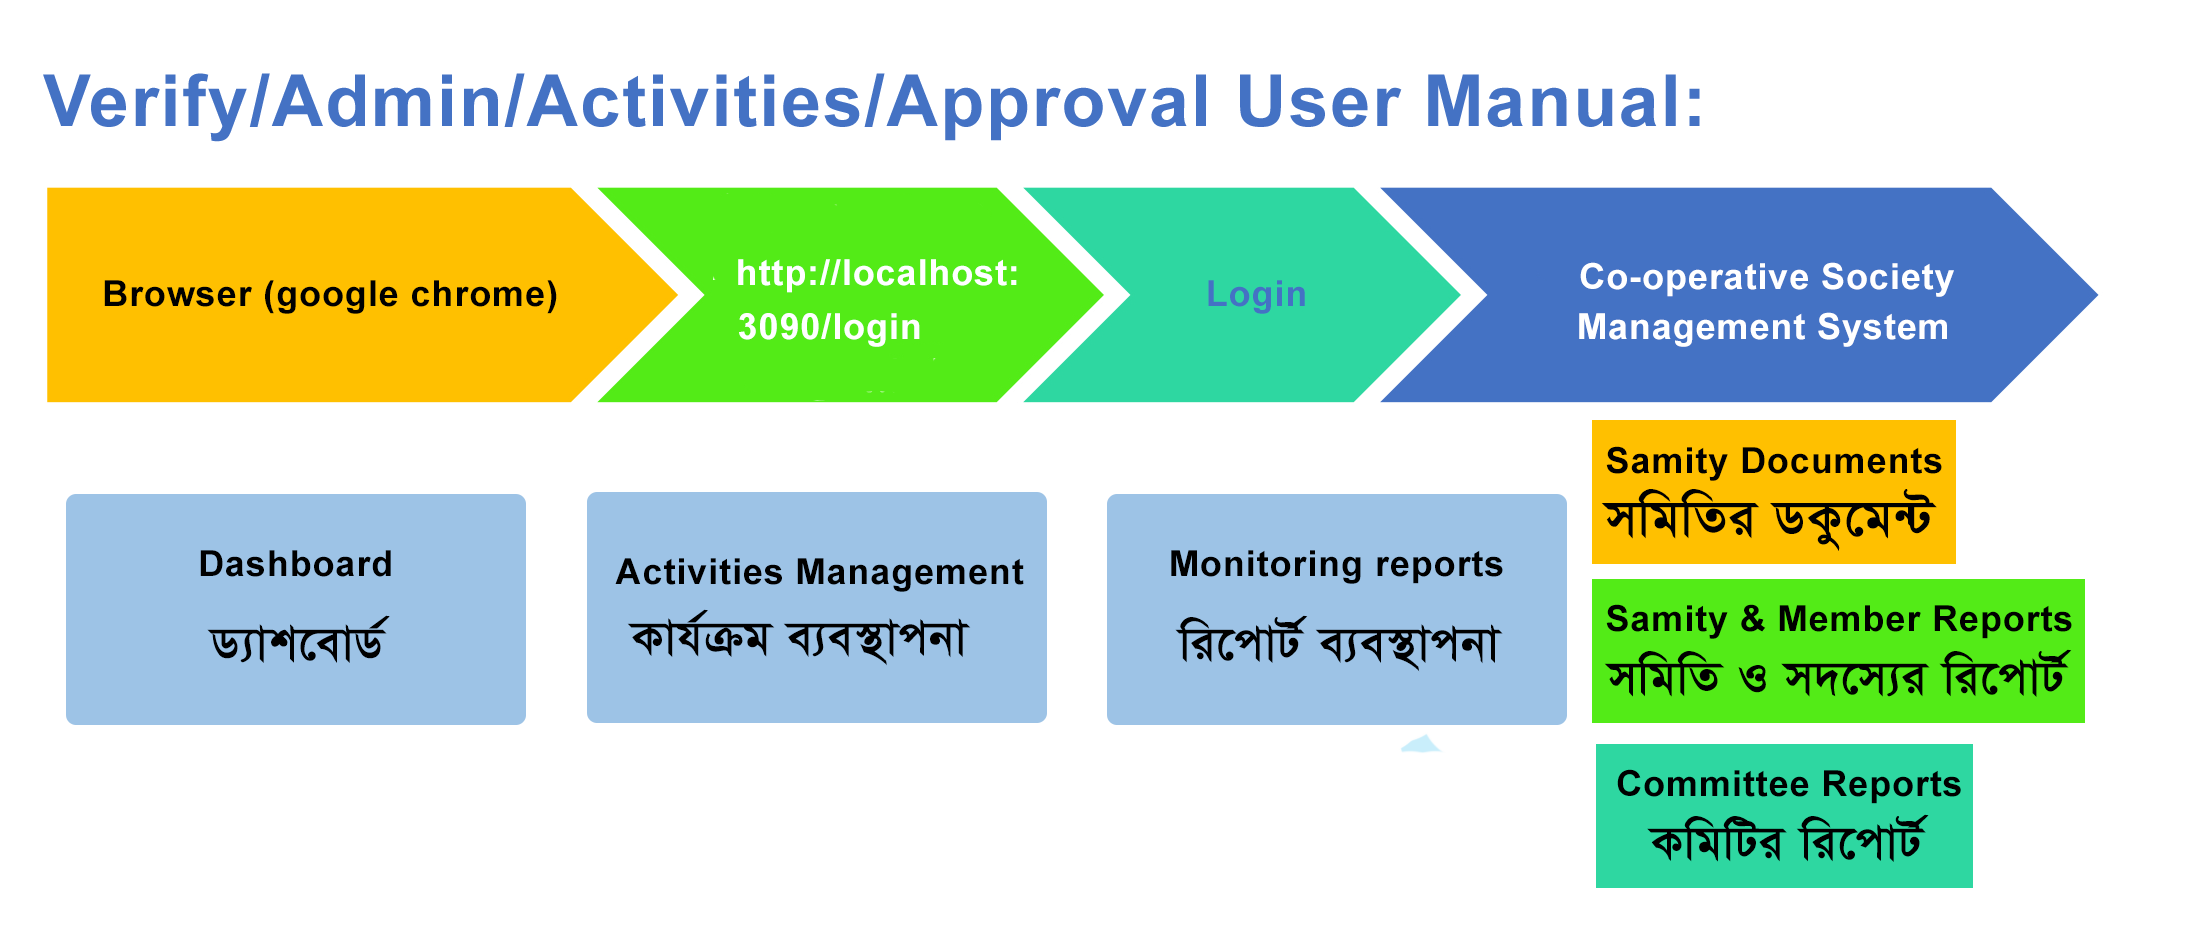
\includegraphics[width=0.6\textwidth]{Chap3/4.png}
  \caption{Entry User Diagram}
  \label{fig:example}
\end{figure}

\begin{figure}[h]
\section{VERIFY/ADMIN/ACTIVITIES/APPROVAL USER }
  \centering
  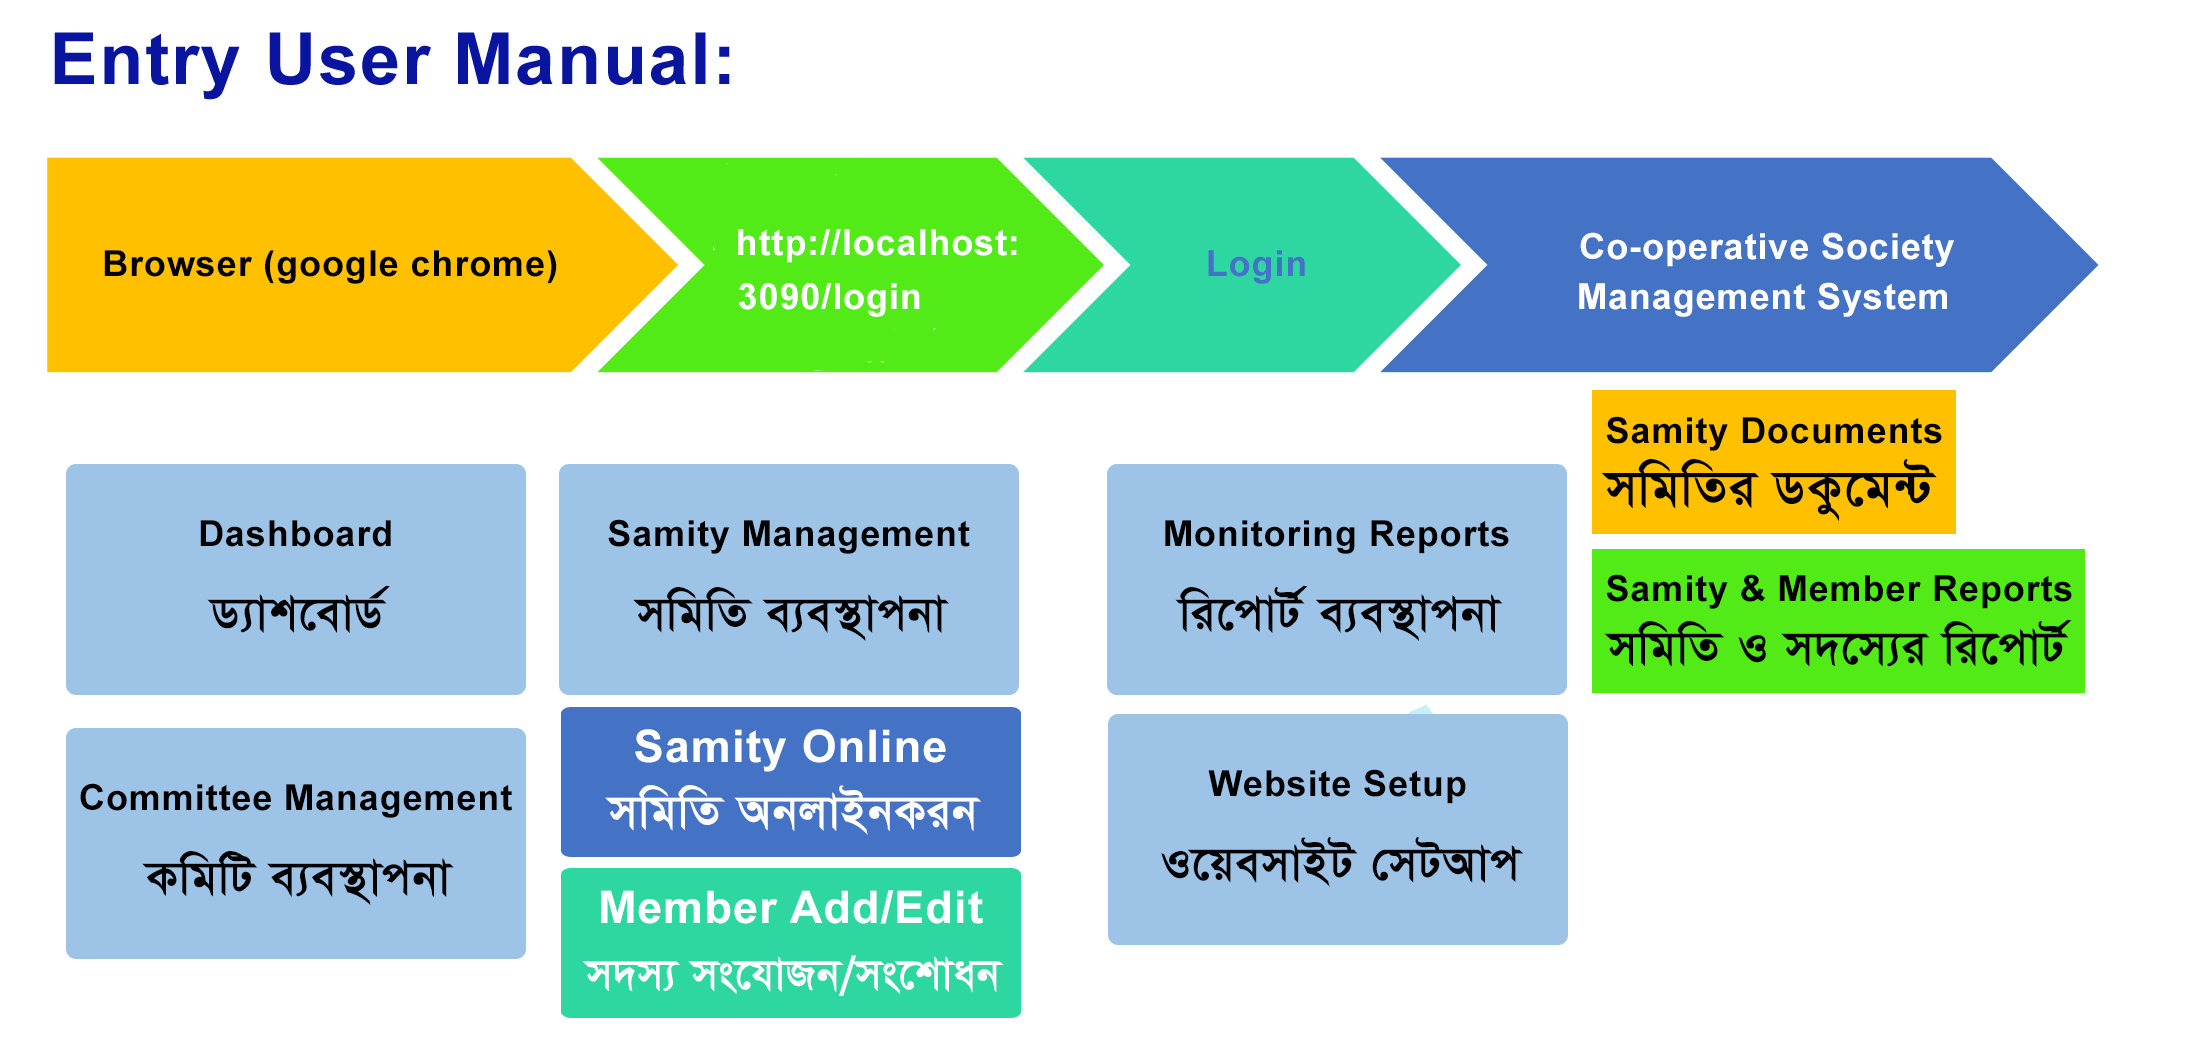
\includegraphics[width=0.6\textwidth]{Chap3/5.png}
  \caption{Verify/Admin/Activities/Approval User Diagram}
  \label{fig:example}
\end{figure}

\begin{figure}[h]
\section{RELATIONAL DATABASE DESIGN}
  \centering
  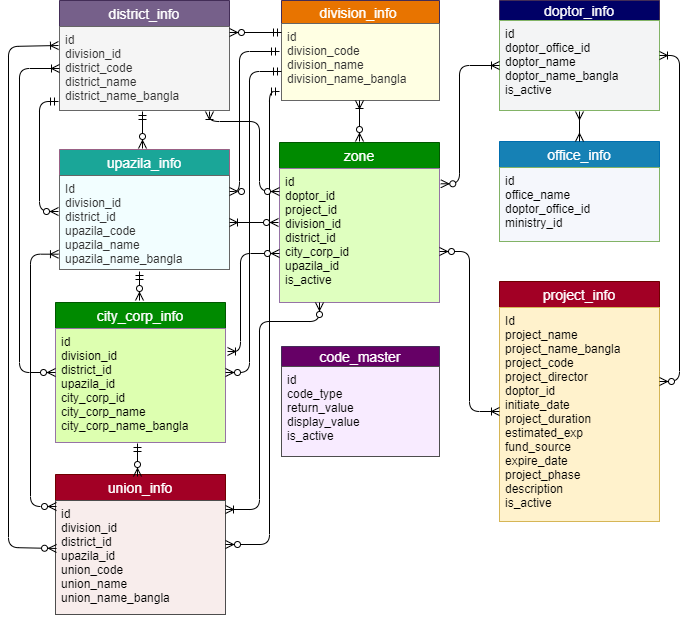
\includegraphics[width=0.6\textwidth]{Chap3/6.png}
  \caption{Zone Setup Database}
  \label{fig:example}
\end{figure}

\begin{figure}[h]
\section{SOCIETY SETUP DATABASE}
  \centering
  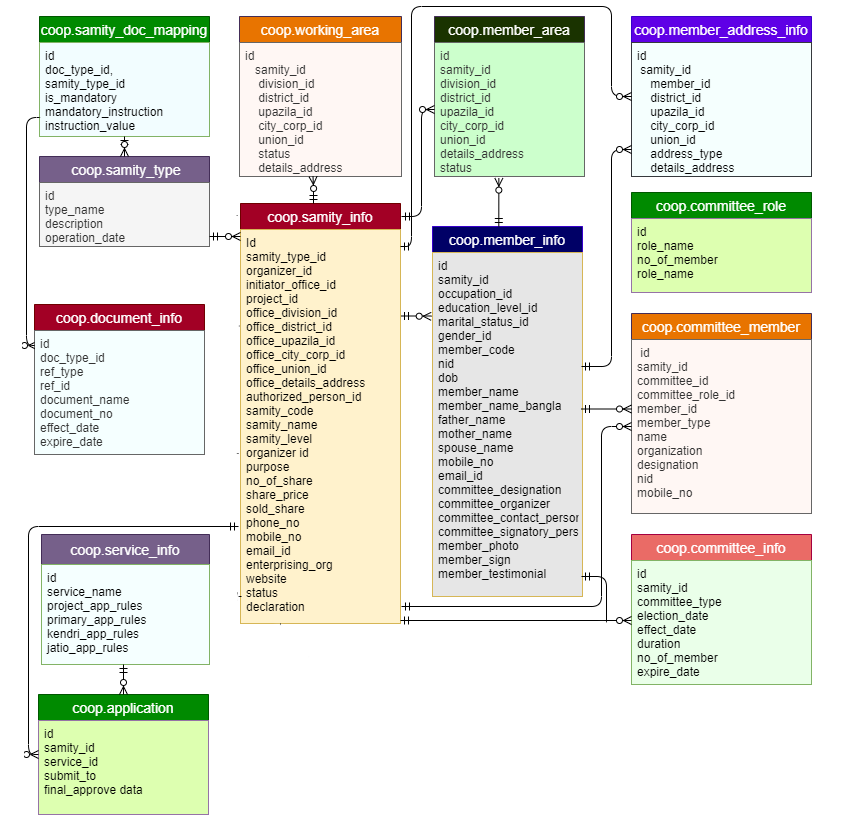
\includegraphics[width=0.6\textwidth]{Chap3/7.png}
  \caption{Society Setup Database}
  \label{fig:example}
\end{figure}

\end{document}

% ////////////////////// image sas ///////////////////////////////
\subsection{IMPLEMENTATION}

Implementing a Co-operative Society Management System involves creating a software 
application that helps manage the various activities and operations of a Co-operative society. 
Here's a basic outline of how you can implement such a system:

\subsubsection*{Dashboard:}
At a glance, show approved, rejected, pending, and waiting societies. It also displays system services based on user roles.

\subsubsection*{Society Management:}
\begin{itemize}
    \item Add and edit societies with documents in this screen by the entry user.
    \item Post to verify user follows up on his activities management and checks information and documents.
    \item Society data on the field is then submitted to the approval user.
    \item Approval user approves the society, then a 19-digit code (Example: 2023.1.01.4161.0001) is generated and stored in the society main table (\texttt{samity\_info}).
\end{itemize}

\subsubsection*{Members Management:}
\begin{itemize}
    \item Two types of entry processes: entry system and excel file upload for approved societies.
    \item Generate an ID for member code and store it in the \texttt{member\_info} table with a relational \texttt{samity\_id}.
\end{itemize}

\subsubsection*{Committee Management:}
\begin{itemize}
    \item Three types of committee types: 
    \begin{enumerate}
        \item Approved First Committee (6-12 members) with a time duration of 2 years.
        \item Elected Committee (6-12 members) with a time duration of 3 years.
        \item Election Committee (3 members) with a time duration of 90 days.
        \item Interim Committee (3 selected members) with a time duration of 45 days.
    \end{enumerate}
    \item Present committee roles as per rules. All data stored in the \texttt{committee\_info} table.
\end{itemize}

\subsubsection*{Website Setup:}
Every society gets one website for society information for Co-operative/Normal users. Set up includes Home, About Us, Members, Services, Project, and Contact of society.

\subsubsection*{Reporting:}
Generate reports on society information, member information, committee information, and overall society performance. Detailed information report attributes link to Jasper Report.



